\documentclass[10pt,a4paper]{article}
\usepackage[utf8]{inputenc}
\usepackage[italian]{babel}
\usepackage{amsmath}
\usepackage{amsfonts}
\usepackage{amssymb}
\usepackage{graphicx}
\usepackage[left=2cm,right=2cm,top=2cm,bottom=2cm]{geometry}
\newcommand{\rem}[1]{[\emph{#1}]}

\author{Gruppo xx \\ Federico Belliardo, Francesco MAzzoncini, Giulia Franchi}
\title{Esercitazione N.5: Transistor JFET.}
\begin{document}

\maketitle

\rem{Aggiungere specificazioni su come si sono coniderati gli rrori nei fit}
\section{Scopo e strumentazione}
Studiare le caratteristiche e realizzare un amplificatore con il JFET a canale N 2N3819.


\section{Studio funzionamento del JFET}
\paragraph{Montaggio e ossevazioni qualitative.}
E' stato montato il circuito in figura \ref{circuito1}, con  $R_1 = 0.994\pm0.008$, $R_2 = 1.95 \pm 0.01$, $V_1 = 15.11\pm0.08 $ e $V_2 = -15.01\pm0.08$. Le due sorgenti di tensione DC ono state ottenute dalle due boccole del generatore in dotazione. $R_2$ è la resistenza totale del potenziometro.

\begin{figure}
\centering
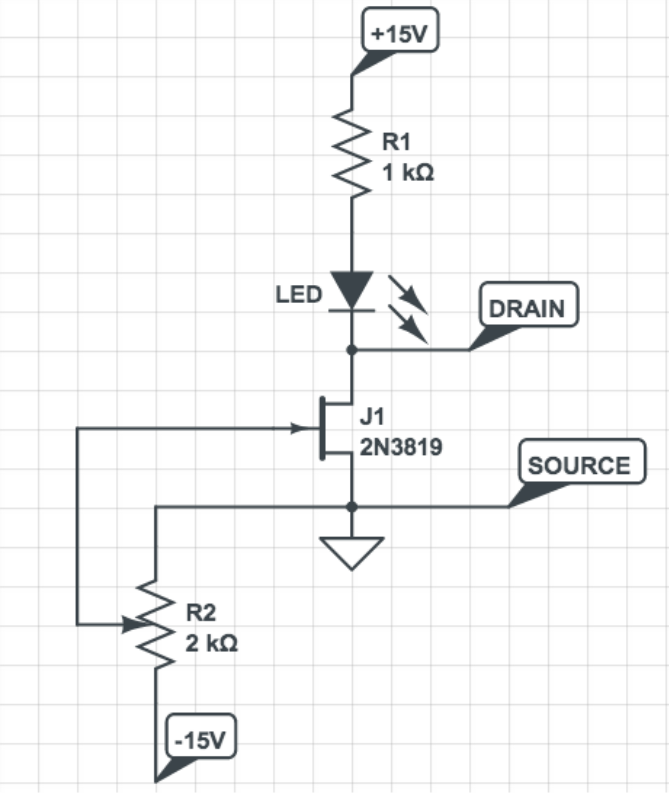
\includegraphics[scale=0.4]{circuito1.png}
\caption{Schema di JFET in corrente continua.\label{circuito1}}
\end{figure}

Variando la resistenza del potenziometro (partitore di tensione) cambia la tensione di \emph{gate} ($V_{GS}$), dunque il JFET entra in conduzione solamente quando si supera la tensione $V_{GS} > V_{P}$ (tensione di \emph{pinch-off}, quando ciò succede si accende il led. Qualitatvamente stimiamo: $V_P = 3.0\pm0.1 \, V$.
\paragraph{Misura della corrente $I_D$ in funzione di $V_GS$.}
Si sono prese misure della tensione $V_{GS}$ e di $V_{R1}$ utilizzando il multimetro digitale (abbiamo evitato l'uso dell'oscilloscopio perchè le nostre misure non fossero affette dall'errore sistematico del $3\%$), da $V_{R1}$ si è ricavata poi $I_D = \frac{V_{R1}}{R_1}$. Nella tabella \ref{correnteId} e in figura \ref{correnteIdVgs} sono riporati i dati presi. \\

\begin{table}[!htb]\centering
\begin{tabular}{|c|c|c|c|}
\hline
$ V_D (V)$ & $ \sigma V_D (V) $ & $V_{GS} (V) $ & $\sigma V_{GS} (V)$\\ 
\hline
0.013 & 0.001 & -3.27 & 0.02\\
0.078 & 0.001 & -3.13 & 0.02\\
0.264 & 0.002 & -2.94 & 0.02\\
0.462 & 0.003 & -2.81 & 0.02\\
1.02 & 0.01 & -2.51 & 0.02\\
1.69 & 0.01 & -2.23 & 0.01\\
2.94 & 0.02 & -1.81 & 0.01\\
4.34 & 0.02 & -1.37 & 0.01\\
6.22 & 0.03 & -0.872 & 0.004\\
8.01 & 0.04 & -0.413 & 0.002\\
9.36 & 0.05 & -0.037 & 0.001\\
\hline
\end{tabular}
\caption{Dati di corrente $I_D$ in funzione delle tensioni $V_{GS}$}
\label{correnteId}
\end{table}

La retta di carico è: $V_1 - R_1 I_D-V_{\gamma}-V_{DS} = 0$ quando scorre corrente $I_D$ (cioè sono in zona ohmica o di saturazione), mentre $V_{DS} = V_1$ quando sono in zona di interdizione.\\

\begin{figure}
\centering
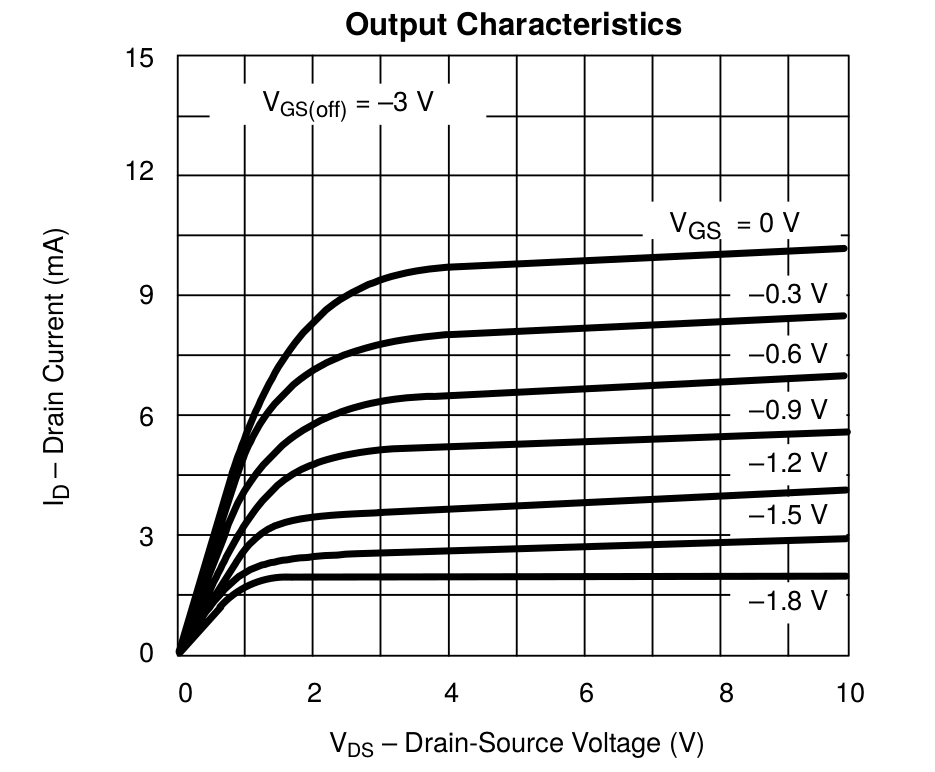
\includegraphics[scale=0.4]{char2.png}
\caption{Curve caratteristiche del JFET dal datasheet.\label{curveCaratteristiche}}
\end{figure}

Il grafico \ref{curveCaratteristiche} riporta un immagine delle curve caratteristiche del JFET nel caso in cui la tensione di \emph{pinch-off} sia $V_P = -2.0 V$, sul quale è riportata la retta di carico. Si vede che per i valori delle tensioni $V_{DS}$ esplorati (calcolati dalla retta di carico e riportati nella tabella \ref{correnteId} siamo sempre in zona di saturazione. 

E' stato eseguito un fit di una funzione parabolica ($I_D = K_P (V_{GS} - V_P)^2$), considerando solamente i dati attorno alla tensione di \emph{pinch-off}, cioè in una regione in cui ci aspettiamo valga il comportamento ideale. 

Per il fit numerico si è utilizzata la funzione \emph{curvefit} della libreria \emph{pylab} con l'opzione \emph{$absolute\,sigma = "true"$}, poichè abbiamo considerando gli errori come statistici, in quanto abbiamo considerato soltanto l'errore di misura sul tester. Riportiamo il grafico in figura \ref{graficoIdVgs} e di seguito parametri fittati con la relativa matrice di covarianza: $K_P = (1.4 \dot 0.8) \dot 10^{-3} \, \frac{A}{V^2}$, $V_P = -3.34 \pm 0.07 \, V$,  $ \Sigma_{ij} = \left( \begin{array}{cc}
7.12 \dot 10^{-7} & 4.09 \dot 10^{-5} \\ 
4.09 \dot 10^{-5} & 4.51 \dot 10^{-3}\\
\end{array} \right)$.

Il punto del grafico per cui $V_{GS} = 0.0V$ corrisponde alla corrente $I_{DSS} = 9.5 \pm 0.1 \, mA $ (stimato), alternativamente si possono utilizzare le informazioni del fit: $I_{DSS} = K_P V_{P}^2 = 15 \pm 10 \, mA$. I due valori non sono campatibili, perchè il fit esguito non può essere estrapolato fino a tensioni prossime allo zero.

\begin{figure}
\centering
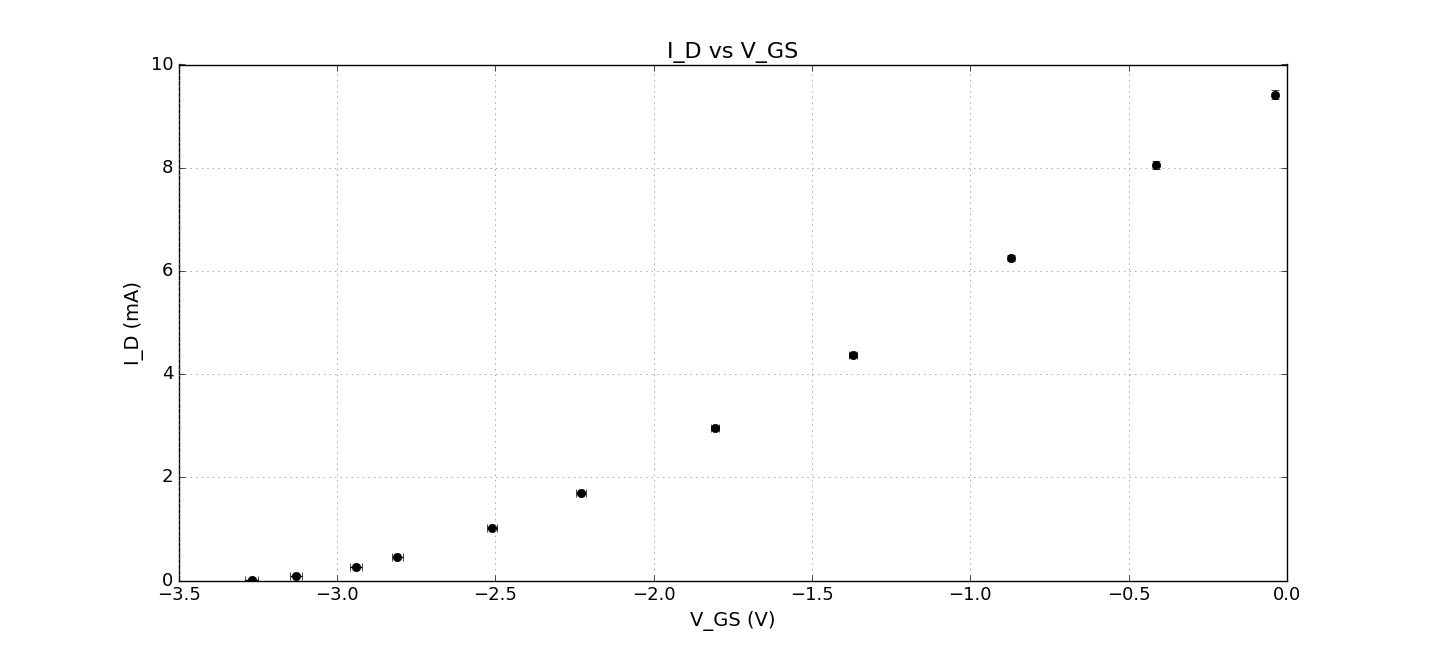
\includegraphics[scale=0.5]{parabolaTutti.png}
\caption{Corrente di drain misurata in funzione della tensione $V_{GS}$.\label{tuttiIdati}}
\end{figure}

\begin{figure}
\centering
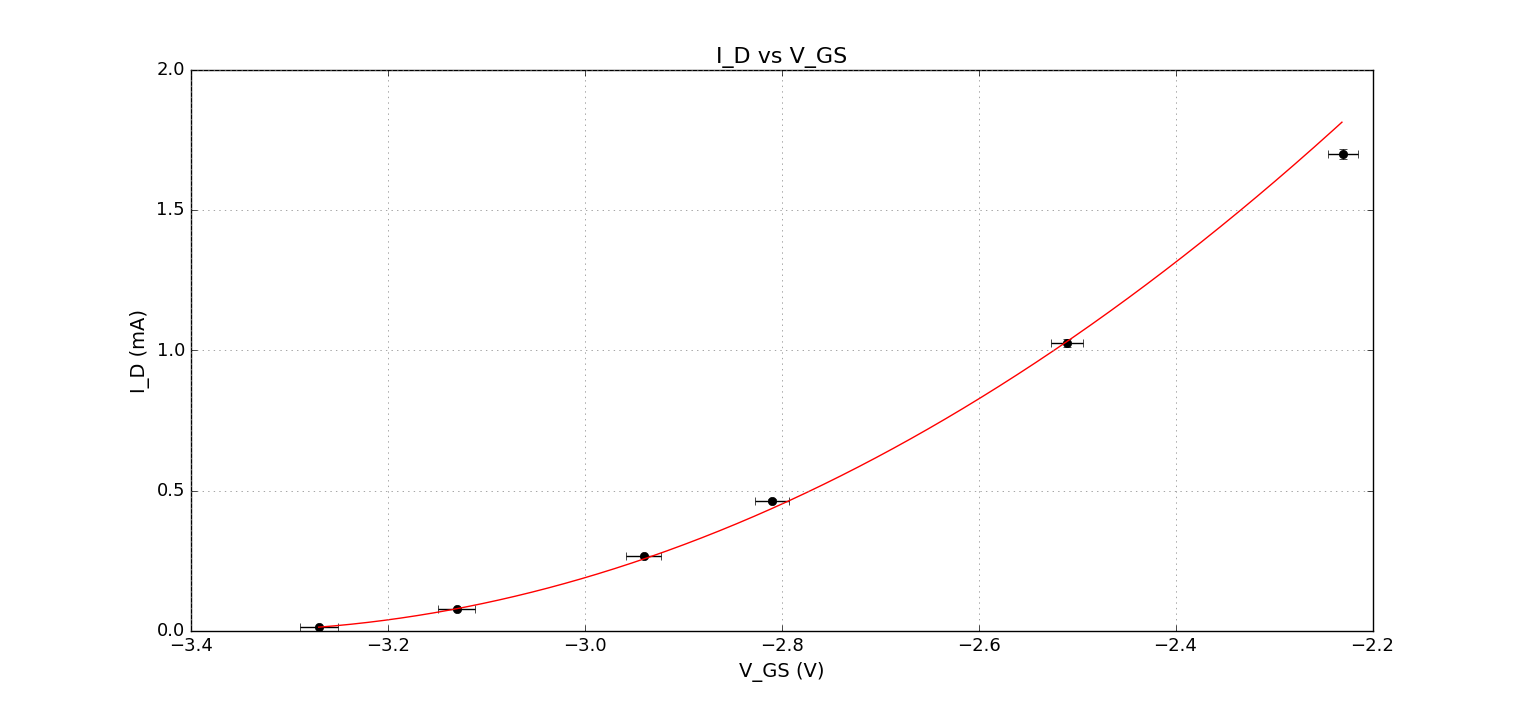
\includegraphics[scale=0.5]{parabolaFit.png}
\caption{Fit parabolico intorno alla tensione di pinch off.\label{correnteIdVgs}}
\end{figure}

Il valore di $V_P$ è molto variabile per costruzione, ma il valore misurato è compatibile con quello tipico indicato nel \emph{datasheet}: $V_{P, datasheet} = -3 \, V$. Per $I_{DSS}$ è riportato un valore tipico di $I_{DSS} = 10 \, mA$ compatibile con quello estratto dal grafico.

\section{Montaggio amplificatore}
\paragraph{Stima della tensione $V_P$ e della corrente $I_DSS$}
Si è montato il circuito in \ref{circuito2}, con i componenti: $R_1 = \pm$, $R_2 = \pm $ e $C_1 = \pm$ e $V_1 = \pm $. Si è regolato il potenziometro in modo che la corrente di quiescenza fosse la metà di $I_{DSS}$, il valore misurato è: $I_D = \pm $. La resistenza a cui si osserva ciò è: $R_{part} = \pm $ (è lasciata costante e sarà usata successivamente). Si è misurata la tensione $V_{GS}$. Dalla formula $V_{GS} = V_{P} \left( 1 - \sqrt{\frac{I_D}{I_{DSS}}} \right)$ (valida in zona di saturazione), ricaviamo il valore atteso per $V_{GS}$ cioè: $V_{GS} =  \pm$.\\ 
Da questi dati si può anche dare una stima della tranconduttanza: $g_m = \frac{i_D}{v_{GS}} = \frac{2I_{DSS}}{\vert V_P \vert} \sqrt{\frac{I_D}{I_{DSS}}} = \pm$. 

\begin{figure}
\centering
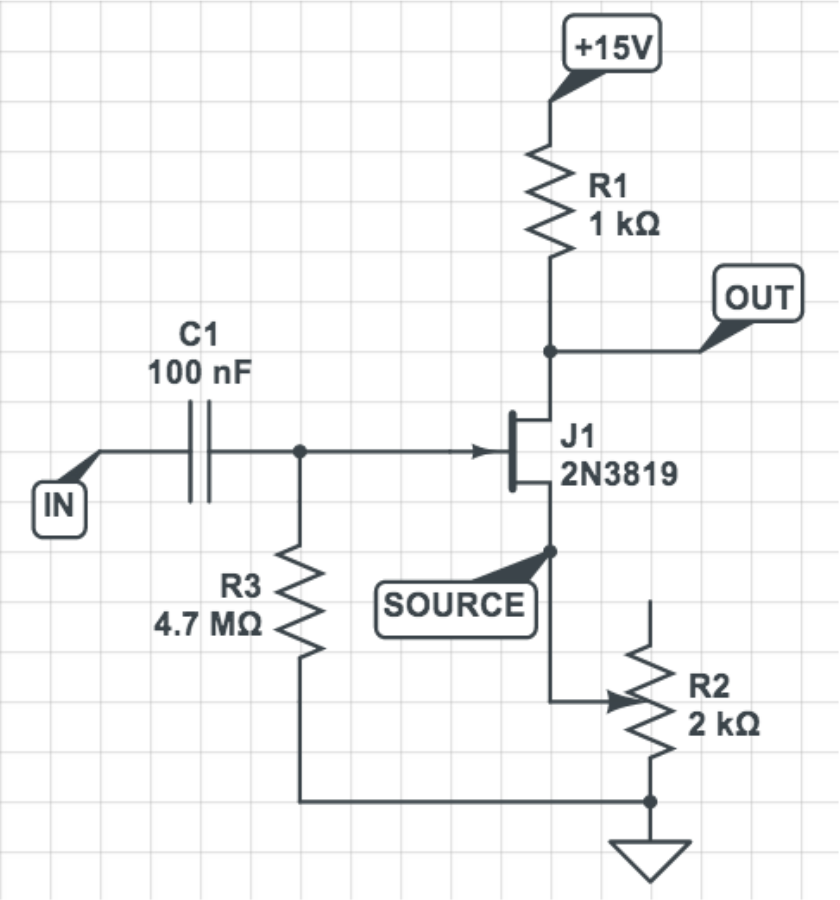
\includegraphics[scale=0.4]{circuito2.png}
\caption{Schema di JFET in corrente continua.\label{circuito2}}
\end{figure}

\section{Misure a frequenza fissa}
Tutte le misure di questa sezione sono prese usando una frequenza fissa di $f_0 = \pm$. L'ingresso del circuito in entrambi i casi è al gate.
\paragraph{Circuito \emph{common source}.}
Si sono prese le misure si tensione in uscita dal \emph{drain}, insieme alle misure di tempo tra un picco del segnale di ingresso e un picco del segnale in uscita. I dati sono riportati nella tabella seguente \ref{tabellaCommonSource}.
\rem{inserire qui la tabella}
Trascuarando la corrente che scorre nel \emph{gate} abbiamo le due eqyuazioni per piccoli segnali: $i_D = g_m v_{gs} = \frac{v_S}{R_{part}}$ e $i_D = g_m v_{gs} = -\frac{v_D}{R_1}$, da queste si ottiene: $A_V = -\frac{v_D}{v_G} = - \frac{R_1 g_m}{1+R_{part} g_m} = \pm $. \rem{Insierire valore numerico}
Come si vede dalla tabella per gli intervalli di tensione per cui si sono prese le misure l'amplificazione rimane circa costante e il suo valore medio è: $A_V = \pm$. \\
Si è iniziato ad avere clipping superiore per $V_{clipping, sup} = \pm $.
\rem{spiegare perchè non c'è clipping inferiore}

\paragraph{Circuito \emph{source follower}.}
Nella tabella \ref{tabellaSourceFollower} sono riportati i dati prendendo come uscita il source, si sono ripetute le stesse misure e analisi.

\rem{inserire la tabella}

Dalle stese equazioni della sezione precedente otteniamo la relazione: $A_V = \frac{R_{part} g_m}{1+R_{part} g_m}$, dalla quale si può stimare teoricamente il guadagno atteso come: $A_V = \pm$. La media delle misure da $A_V = \pm$. I due valori sono in accordo entro l'errore sperimentale.

Si osserva clipping inferiore alla tensione: $V_{clipping, inf} = \pm $. 
\rem{Spiegare perchè non si ha clipping superiore}

\rem{vedere se mettere l'immagine del modello a piccoli segnali, soprattuto quale mettere...}

Nella formula per determinare il guadagno vediamo $g_m$ sia a numeratore che a denominatore, duqnue non possiamo propagare l'errore considerandoli come indipendenti (sovrastimeremmo troppo l'errore sull'amplificazione). L'errore è stato propagato considerando la semidispersione massima ($\Delta = A_V(<g_m> + \sigma g_m, R_1, R_{part}) - A_V(<g_m> - \sigma g_m, R_1, R_{part})$) sommata in quadratura con l'errore ottenuto propagando $\sigma R_1$ e $\sigma R_{part}$ come errori statisticamente indipendenti.
In realtà la propagazione statistica eseguita con le derivate parziali (di $A_V(g_m, R_1, R_{part})$) sommate in quadratura già li considera come errori non indipendenti, quindi è possibile utilizzare le librerie \emph{uncertainties}
\section{Misura impedenza di ingresso}
Trascurando le impedenze tra i terminali del JFET possiamo stimare $R_{int} = \frac{1}{j \omega C} + R_3 \sim R_3 = \pm$. Per eseguire la misura si sono misurate le uscite con e senza resistenza $R_{S}$ posta in serie al generatore di funzioni. La resistenza in ingresso attesa si ottiene dalla formula del partitore di tensione, $\frac{R_S}{R_IN} = \frac {V_1}{V_2} - 1$ (dove $V_1$ è la tensione misurata senza resistenza $R_S$). Si sono ripetute le misure per le frequenze $f_1 = 1 kHz$ e $f_2 = 10 kHz$.

In tabella sono anche riportate le frequenze attese calcolate teoricamente alle due frequenze:\\

\begin{tabular}{|c|c|c|c|c|}
\hline 
• & $V_1$ & $V_2$ & $R_{IN}$ & $R_{IN, att}$ \\ 
\hline
$1 kHz$ & • & • & • & • \\ 
\hline 
$10 kHz$ & • & • & • & • \\ 
\hline 
\end{tabular}\\

L'impedenza misurata sperimentalmente è minore di quella calcolata teoricamente a causa delle impendenze delle capacità tra i terminali del JFET, che sono poste in parallelo alla resistenzea $R_3$.

\section{Aumento del guadagno}
In questa sezine si è mantenta costante la frequenza di lavoro e variando il potenziometro si sono effettuate diverse misure di tensione in uscita. \rem{abbiamo dovuto verificare che l'ingresso fosse costante?}. Il valore massimo del guadagno è risultato essere quello per cui la resistenza $R_S$ era minore (teoricamente nulla) ($R_{S, min}$). Il valore teorico del guadagno con questa resistenza è: $A_V = \pm $, che non è compatibile con il valore misurato.

\end{document}